In this paper, we focus on settings where the supervision signal from denotations is especially weak.  In the Cornell Natural Language Visual Reasoning dataset (NLVR)~\citep{suhr2017corpus}, for instance, each utterance is a statement that is labeled as either true or false.  Because this supervision signal is binary, roughly half of all possible logical forms will evaluate to the correct answer, and so naive approaches to learning from denotations do not perform well.

We introduce two innovations to improve learning from denotations, motivated by these particularly weak supervision settings, but applicable to any semantic parser trained only on denotations.  The first is to include a notion of coverage over the question to guide the training algorithm towards logical forms that not only evaluate to the correct denotation, but also have some connection to the words in the utterance.

Our second contribution is an iterative procedure for refining a set of candidate logical forms for each training instance, leading to better training data and better parsing accuracy.  We interleave the use of a maximum marginal likelihood training objective with a structured learning algorithm.  After the structured learning algorithm converges, we use the trained model to find the most likely logical forms that evaluate to the correct denotation, and we use these denotations to train a new model with a maximum marginal likelihood objective, this iteratively increasing the coverage of logical forms in the training data and their complexity.

We demonstrate the effectiveness of these two contributions on two difficult reasoning tasks: NLVR and \WTQ~\citep{pasupat2015compositional}.  Our contributions improve a weakly-supervised semantic parser from essentially random performance to 82.9\% accuracy on NLVR, establishing a new state-of-the-art result.  On \WTQ{}, our iterative training algorithm improves the accuracy of a baseline parser by 6\% absolute.

\section{Type-constrained decoding for semantic parsing} \label{sec:type_constrained_decoding}
In this work, we use a type-constrained encoder-decoder neural semantic parser for our experiments.  Of the many variants of this basic architecture (see \secref{sec:related_work}), all of which are essentially seq2seq models with constrained outputs and/or re-parameterizations, we choose to use the parser of \citet{krishnamurthy2017neural}, as it is particularly well-suited to the \WTQ{} dataset, which we evaluate on.

The encoder in the model is a bi-directional recurrent neural network with Long Short-Term Memory (LSTM) \citep{hochreiter1997long} cells, and the decoder is a grammar-constrained decoder also with LSTM cells.  Instead of directly outputting tokens in the logical form, the decoder outputs \emph{production rules} from a CFG-like grammar.  These production rules sequentially build up an abstract syntax tree, which determines the logical form.  The model also has an entity linking component for producing table entities in the logical forms; this component is only applicable to \WTQ{}, and we remove it when running experiments on NLVR.  The particulars of the model are not the focus of this work, so we refer the reader to the original paper for more details.

\section{Datasets} \label{sec:datasets}
We will now describe the two datasets we use in this work to evaluate our methods -- Cornell NLVR and \WTQ.
\subsection{Cornell NLVR}
Cornell NLVR is a language-grounding dataset containing natural language sentences provided along with synthetically generated visual contexts, and a label for each sentence-image pair indicating whether the sentence is true or false in the given context. 
\begin{figure}
	\centering
		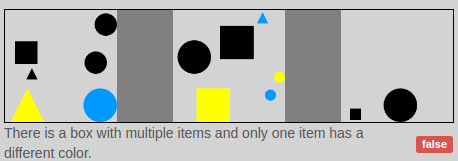
\includegraphics[width=3in]{figures/nlvr_example.png}
		    \caption{Example from NLVR dataset showing one sentence associated with two worlds and corresponding binary labels, and translation of the sentence above in our logical form language.}
			\label{fig:nlvr_example}
\end{figure}
Figure~\ref{fig:nlvr_example} shows two example sentence-image pairs from the dataset (with the same sentence). The dataset also comes with structured representations of images, indicating the color, shape, size, and x- and y-coordinates of each of the objects in the image. While we show images in Figure~\ref{fig:nlvr_example} for ease of exposition, we use the structured representations in this work.

Following the notation introduced in \secref{sec:semantic_parsing}, $x_i$ in this example is \textit{There is a box with only one item that is blue}. The structured representations associated with the two images shown are two of the worlds ($w^1_i$ and $w^2_i$), in which $x_i$ could be evaluated. The corresponding labels are the denotations $d^1_i$ and $d^2_i$ that a translation $y_i$ of the sentence $x_i$ is expected to produce, when executed in the two worlds respectively. That the same sentence occurs with multiple worlds is an important property of this dataset, and we make use of it in defining the training objective of our parser (see \secref{sec:coverage_guided_search}).
\subsection{Logical form languages} \label{sec:logical_form_languages}

For NLVR, we define a typed variable-free functional query language, inspired by the GeoQuery language \citep{zelle1996learning}. Our language contains six basic types: \texttt{box} (referring to one of the three gray areas in Figure~\ref{fig:nlvr_example}), \texttt{object} (referring to the circles, triangles and squares in Figure~\ref{fig:nlvr_example}), \texttt{shape}, \texttt{color}, \texttt{number} and \texttt{boolean}. The constants in our language are color and shape names, the set of all boxes in an image, and the set of all objects in an image. The functions in our language include those for filtering objects and boxes, and making assertions, a higher order function for handling negations, and a function for querying objects in boxes. This type specification of constants and functions gives us a grammar with 115 productions, of which 101 are terminal productions (see Supplemental Material for the complete set of rules in our grammar). Figure~\ref{fig:nlvr_example} shows an example of a complete logical form in our language.

\section{Coverage-guided search}\label{sec:coverage_guided_search}

Weakly-supervised training of semantic parsers relies heavily on lexical cues to guide the initial stages of learning to good logical forms.  Traditionally, these lexical cues were provided in the parser's lexicon.  Neural semantic parsers remove the lexicon, however, and so need another mechanism for obtaining these lexical cues.  In this section we introduce the use of coverage to inject lexicon-like information into neural semantic parsers.

Coverage is a measure of relevance of the candidate logical form $y_i$ to the input $x_i$, in terms of how well the productions in $y_i$ map to parts of $x_i$. We use a small manually specified lexicon as a mapping from source language to the target language productions, and define coverage of $y_i$ as the number of productions triggered by the input utterance, according to the lexicon, that are included in $y_i$. The lexicon contains under 40 rules, mainly mapping words and phrases to constants and unary functions in the target language. The complete lexicon is shown in the supplemental material. As an example, the target language productions triggered by the sentence in Figure~\ref{fig:nlvr_example} are \texttt{box\_exists}, \texttt{1} and \texttt{color\_blue}. We find that a small but precise lexicon is sufficient to guide the search process away from spurious logical forms. Moreover, as shown empirically in \secref{sec:results_coverage}, the model does not learn much without this simple but crucial guidance.

We use this measure of coverage to augment our loss function during training.  When using expected risk minimization to train our model (see \secref{sec:erm}) we include coverage in the cost function $\mathcal{C}$:
\begin{equation}
	\mathcal{C}(x_i, y_i, W_i, D_i) = \lambda \mathcal{S}(y_i, x_i) + \\
		(1 - \lambda)\mathcal{T}(y_i, W_i, D_i)
		\label{eq:cost}
\end{equation}
where the function $\mathcal{S}$ measures the number of items that $y_i$ is missing from the the actions triggered by the input utterance $x_i$ given the lexicon, the function $\mathcal{T}$ measures the consistency of the evaluation of $y_i$ in $w_i$, and $\lambda$ is a hyper-parameter.  $\mathcal{T}$ is formally defined as
\begin{equation}
	\mathcal{T}(y_i, W_i, D_i) = \begin{cases}
		0 &\text{if } \forall_{\substack{w^j_i \in W_i\\d^j_i \in D_i}} \llbracket y_i \rrbracket^{w^j_i} = d^j_i\\
		e &\text{otherwise}
	\end{cases}
	\label{eq:consistency}
\end{equation}
We set $e$ as the maximum possible value of the coverage cost for the corresponding instance, to make the two costs comparable in magnitude.

\subsection{Coverage-guided constrained decoding}
We additionally slightly modify the constrained decoding architecture described in \secref{sec:semantic_parsing} to bias the predicted actions towards those that would decrease the value of $\mathcal{S}(y_i, x_i)$. This is done using a coverage vector, $v^{\mathcal{S}}_i$ for each training instance that keeps track of the production rules triggered by $x_i$, and gets updated whenever one of those desired productions is produced by the decoder. That is, $v^{\mathcal{S}}_i$ is a vector of 1s and 0s, with 1s indicating the triggered productions that are yet to be produced by the decoder. This is similar to the idea of checklists used by \citet{kiddon2016globally}. The decoder in the original architecture scores output actions at each time step by computing a dot product of the predicted action representation with the embeddings of each of the actions. We add a weighted sum of all the actions that are yet to produced:
\begin{equation}
	s^a_i = e^a . (p_i + \gamma * v^{\mathcal{S}}_i . E)
\end{equation}
where $s^a_i$ is the score of action $a$ at time step $i$, $e^a$ is the embedding of that action, $p_i$ is the predicted action representation, $E$ is the set of embeddings of all the actions, and $\gamma$ is a learned parameter for regularizing the bias towards yet-to-be produced triggered actions.

\section{Iterative search and maximization} \label{sec:iterative_search}
\begin{algorithm}[h!]
	\SetAlgoLined
	\SetKwInOut{Input}{Input}
	\SetKwInOut{Output}{Output}
	\Input{Dataset $\mathcal{D} = \{X, W, D\}$; and \\
	seed set $\mathcal{D}^0 = \{X^0, Y^0\}$ such that \\
	$X^0 \subset X$ and $\mathcal{C}(x^0_i, y^0_i, W_i, D_i) =0$} 
	\Output{Model parameters $\theta^{\texttt{ERM}}$}
	Initialize dataset $\mathcal{D}^{\texttt{MML}} = \mathcal{D}^0$\;
	\While{$\text{Acc}(\mathcal{D}_{\text{dev}})$ is increasing}{
		$\theta^{\texttt{MML}} = \texttt{MML}(\mathcal{D}^{\texttt{MML}})$\;
		Initialize $\theta^{\texttt{ERM}} = \theta^{\texttt{MML}}$\;
		Update $\theta^{\texttt{ERM}} = \texttt{ERM}(\mathcal{D}; \theta^{\texttt{ERM}})$\;
		Update $\mathcal{D}^{\texttt{MML}} = \texttt{Decode}(\mathcal{D}; \theta^{\texttt{ERM}})$\;
	}
	\caption{Iterative coverage-guided search}\label{alg:iterative_search}
\end{algorithm}

In this section we describe the second contribution of this work, which is an iterative technique for refining the set of candidate logical forms associated with each training instance.

As discussed in \secref{sec:prior_training}, most prior work on weakly-supervised training of semantic parsers uses dynamic MML.  This is particularly problematic in domains like NLVR, where the supervision signal is binary---it is very hard for dynamic MML to bootstrap its way to finding good logical forms.  To solve this problem, we interleave static MML, which has a consistent supervision signal from the start of training, with a dynamic learning algorithm.  We use coverage-augmented ERM instead of dynamic MML; recall, however, that the two learning algorithms have a strong similarity (see \secref{sec:erm}).

\begin{table*}
	\centering
	\begin{tabular}{lcccccc}
	\toprule
	\multicolumn{1}{c}{} & \multicolumn{2}{c}{Dev.} & \multicolumn{2}{c}{Test-P} & \multicolumn{2}{c}{Test-H} \\
	Model & Acc. & Cons. & Acc. & Cons. & Acc. & Cons.\\
	\midrule
	MaxEnt \citep{suhr2017corpus} & 68.0 & - & 67.7 & - & 67.8 & - \\
	BiATT-Pointer \citep{tan2018object} & 74.6 & - & 73.9 & - & 71.8 & - \\
	Abs. Sup. \citep{goldman2017weakly} & 84.3 & 66.3 & 81.7 & 60.1 & - & - \\
	Abs. Sup. + ReRank \citep{goldman2017weakly} & 85.7 & 67.4 & 84.0 & 65.0 & 82.5 & 63.9 \\
	This work & 85.4 & 64.8 & 82.4 & 61.3 & \textbf{82.9} & \textbf{64.3} \\
	\bottomrule
	\end{tabular}
	\caption{Comparison of our model with previously published models. We show accuracy and consistency on the development set, and public (Test-P) and hidden (Test-H) test sets.}\label{tab:main_result}
\end{table*}

In order to use static MML, we need an initial set of candidate logical forms.  We obtain this candidate set using a bounded-length exhaustive search, filtered using heuristics.  A bounded-length search will not find logical forms for the entire training data, so we can only use a subset of the data for initial training.  We train a model to convergence using static MML on these logical forms, then use that model to initialize coverage-augmented ERM training.  This gives the model a good starting place for the dynamic learning algorithm, and the search at training time can look for logical forms that are longer than could be found with the bounded-length exhaustive search.  We train ERM to convergence, then use beam search on the ERM model to find a new set of candidate logical forms for static MML on the training data.  This set of logical forms can have a longer length than the initial set, because the search is no longer exhaustive, and will thus likely cover more of the training data.  In this way, we can iteratively improve the candidate logical forms used for static training, which in turn improves the starting place for the structured learning algorithm.

Algorithm~\ref{alg:iterative_search} concretely describes this process. \texttt{Decode} in the algorithm refers to running a beam search decoder that returns a set of consistent logical forms (i.e. $\mathcal{T} = 0$) for each of the input utterances. We start off with a seed dataset $\mathcal{D}^0$ for which consistent logical forms are available.

\section{Experiments} \label{sec:experiments}

We evaluate both our contributions on NLVR. Furthermore, to evaluate how well \emph{iterative search and maximization} extends to domains with non-binary denotation labels, we test on \WTQ{} as well.

\subsection{Experimental setup}
\paragraph{NLVR} We use the standard train-dev-test split for NLVR, containing 12409, 988 and 989 sentence-image pairs respectively. NLVR contains most of the sentences occurring in multiple worlds (with an average of 3.9 worlds per sentence), and we use this property by defining the consistency cost, $\mathcal{T}$ of a logical form $y_i$ in Equation~\ref{eq:consistency} to be 0 only if its denotation in all the corresponding worlds is correct. While training the model, we set the word embedding and action embedding sizes to 50, and the hidden layer size of both the encoder and the decoder to 30. We initialized all the parameters, including the word and action embeddings using Glorot uniform initialization \citep{glorot2010understanding}. We found that using pretrained word representations did not help. We added a dropout \citep{srivastava2014dropout} of 0.2 on the outputs of the encoder and the decoder and before predicting the next action, set the beam size to 10 both during training and at test time, and trained the model using ADAM \citep{kingma2014adam} with a learning rate of 0.001. All the hyper-parameters are tuned on the validation set. 

For our iterative search algorithm, we obtain an initial set of candidate logical forms by exhaustively searching to a depth of 10\footnote{It was prohibitively expensive to search beyond depth of 10, and even bounding the value at 10 resulted in more than 800k logical forms.}. We use the coverage lexicon described in \secref{sec:coverage_guided_search} for the search, and retrieve logical forms that have full coverage according to the lexicon, and also lead to the correct denotations in all the corresponding worlds. That is, we retrieve logical forms for which $\mathcal{C} = 0$. This process results in logical forms for 51\% of the sentences in train and dev sets.

At each iteration of the search step in our iterative training algorithm, we increase the maximum depth of our search with a step-size of 2, finding more complex logical forms and covering a larger proportion of the training data. While exhaustive search is prohibitively expensive beyond a fixed number of steps, our training process that uses beam search based approximation can go deeper.

\paragraph{\WTQ} This dataset comes with five different cross-validation folds of training data, each containing a different 80/20 split for training and development. In \secref{sec:results_iterative}, we show results on the first fold. We replicate the model presented in \citet{krishnamurthy2017neural}, and only change the training algorithm.  For our initial set of candidate logical forms, we use the result of dynamic programming on denotations \cite{pasupat2016inferring}, which was also used by \cite{krishnamurthy2017neural}.


\subsection{Main Results}
In Table~\ref{tab:main_result}, we show a comparison of the performance of our \textit{iterative coverage-guided search} algorithm with the previously published approaches for NLVR. The first two rows correspond to models that are not semantic parsers. This shows that semantic parsing is a promising direction for this task. The closest work to ours is the weakly supervised parser built by \cite{goldman2017weakly}. They build a lexicon similar to ours for mapping surface forms in input sentences to abstract clusters. But in addition to defining a lexicon, they also manually annotate complete sentences in this abstract space, and use those annotations to perform data augmentation for training a supervised parser, which is then used to initialize a weakly supervised parser. They also explicitly use the abstractions to augment the beam during decoding using caching, and a separately-trained discriminative re-ranker to re-order the logical forms on the beam.  As a discriminative re-ranker is orthogonal to our contributions, we show their results with and without it, with ``Abs. Sup.'' being more comparable to our work. Our model, which uses no data augmentation, no caching during decoding, and no discriminative re-ranker, outperforms their variant without reranking on the public test set, and outperforms their best model on the hidden test set, achieving a new state-of-the-art result on this dataset.

\begin{table}
	\centering
	\begin{tabular}{lcccc}
	\toprule
	\multicolumn{1}{c}{}& \multicolumn{2}{c}{No coverage} & \multicolumn{2}{c}{+ coverage} \\
	\multicolumn{1}{c}{}& Acc. & Cons. & Acc. & Cons. \\
	\midrule
	No init.  & 56.4 & 12.0 & 73.9 & 43.6 \\
	MML init. & 77.7 & 51.1 & 80.7 & 56.4 \\
	\bottomrule
	\end{tabular}
	\caption{Effect of coverage guidance on NLVR parsers trained with and without initialization from an MML model. Metrics shown are accuracy and consistency on the public test set.}\label{tab:coverage_guidance}
\end{table}

\subsection{Coverage-guided search} \label{sec:results_coverage}
To evaluate the first contribution of this work, we compare the the performance of the NLVR parser in two different settings: with and without coverage guidance in the cost function. We also compare the performance of the parser in the two settings, when initialized with parameters from an MML model trained to maximize the likelihood of the set of logical forms obtained from exhaustive search. Table~\ref{tab:coverage_guidance} shows the results of this comparison. We measure accuracy and consistency of all four models on the publicly available test set, using the official evaluation script. Consistency here refers to the percentage of logical forms that produce the correct denotation in all the corresponding worlds, and is hence a stricter metric than accuracy. The cost weight ($\lambda$ in Equation~\ref{eq:cost}) was tuned based on validation set performance for the runs with coverage, and we found that $\lambda = 0.4$ worked best.

It can be seen that both with and without initialization, coverage guidance helps by a big margin, with the gap being even more prominent in the case where there is no initialization. When there is neither coverage guidance nor a good initialization, the model does not learn much from unguided search and get a test accuracy not much higher than the majority baseline of 56.2\%.

\begin{table}
	\centering
	\begin{tabular}{llcc}
	\toprule
	Iteration & \% cov. & Step & Dev. Acc  \\
	\midrule
	0 & 51 & M & 64.0 \\
	\hline
	\multirow{2}{*}{1} & \multirow{2}{*}{65} & S & 81.6  \\
	& &  M & 76.5  \\
	\hline
	\multirow{2}{*}{2} & \multirow{2}{*}{65} & S & 82.7  \\
	& &  M & 81.8  \\
	\hline
	\multirow{2}{*}{3} & \multirow{2}{*}{73} & S & 85.4  \\
	& &  M & 83.1  \\
	\hline
	\multirow{2}{*}{4} & \multirow{2}{*}{75} & S & 84.7  \\
	& &  M & 81.2  \\
	\bottomrule
	\end{tabular}
	\caption{Effect of iterative search (S) and maximization (M). \% cov. is the percentage of training data for which the S step retrieves consistent logical forms.}\label{tab:iterative_search_nlvr}
\end{table}

\begin{table}
	\centering
	\begin{tabular}{lccc}
	\toprule
	Iteration & Step & Dev & Test \\
	\midrule
	0 & M & 35.8 & 35.4 \\
	\hline
	\multirow{2}{*}{1} & S & 38.8 & 39.0  \\
	& M & 41.0 & 41.2  \\
	\hline
	2 & S & 40.6 & 41.3 \\
	\bottomrule
	\end{tabular}
	\caption{Iterative search on \WTQ{}.  M and S refer to Maximization and Search steps.}\label{tab:iterative_search_wtq}
\end{table}

\begin{table*}
	\centering
	\begin{tabular}{cl}
	\multirow{2}{*}{0} & \textit{There is a tower with four blocks}\\
	& \texttt{(box\_exists (member\_count\_equals all\_boxes 4))}\\
	\multirow{2}{*}{1} & \textit{Atleast one black triangle is not touching the edge}\\
	& \texttt{(object\_exists (black (triangle ((negate\_filter touch\_wall)} \\
	& \texttt{all\_objects))))}\\
	\multirow{2}{*}{2} & \textit{There is a yellow block as the top of a tower with exactly three blocks.} \\
	& \texttt{(object\_exists (yellow (top (object\_in\_box} \\
	& \texttt{(member\_count\_equals all\_boxes 3)))))}\\
	\multirow{3}{*}{3} & \textit{There is a box with only two black and blue items.} \\
	& \texttt{(box\_exists (member\_color\_any\_equals (member\_color\_any\_equals }\\
	& \texttt{(member\_count\_equals all\_boxes 2) color\_blue) color\_black))}\\ 
	\end{tabular}
	\caption{Complexity of logical forms produced at different iterations, from iteration 0 to iteration 3}\label{tab:logical_form_complexity}
\end{table*}
\subsection{Iterative search and maximization} \label{sec:results_iterative}
To evaluate the effect of \textit{iterative search and maximization}, we present the accuracy numbers from the search (S) and maximization (M) steps from different iterations in Table~\ref{tab:iterative_search_nlvr}. Additionally, we also show the percentage of sentences in the training data for which we were able to obtain consistent logical forms from the S step in each of the iterations, the set that was be used in the M step of the same iteration. It can be seen from the trend for NLVR in Table~\ref{tab:iterative_search_nlvr} that a better MML model gives a better initialization for ERM, and a better ERM model results in a larger set of utterances for which we can retrieve consistent logical forms, thus improving the subsequent MML model.

To test whether iterative training is applicable to other semantic parsing domains with weak supervision, we also evaluate the technique on \WTQ. We apply our iterative technique, without the coverage-augmented cost, to a re-implementation of the parser of \citet{krishnamurthy2017neural}.\footnote{The logical forms used for training, obtained from \citet{pasupat2016inferring}, already provide strong lexical cues to the parser, making a coverage term largely unnecessary.}  Our re-implementation does not yet match the accuracy of the original parser, but it is close enough to demonstrate the effectiveness of our method.  Using two iterations of our iterative search technique, accuracy improves from 35.4\% to 41.3\%, an increase of 6\% absolute.  Table~\ref{tab:iterative_search_wtq} shows these results.

\paragraph{Complexity of Logical Forms} We analyzed the logical forms produced by our iterative search algorithm at different iterations to see how they differ. As expected, for NLVR, allowing greater depths lets the parser explore more complex logical forms. Table~\ref{tab:logical_form_complexity} shows examples from the validation set that indicate this trend.

\section{Conclusion}
We have presented a new technique for training semantic parsers with weak supervision.  Our key insights are that lexical cues are crucial for guiding search during the early stages of training, and that the particulars of the approximate marginalization in maximum marginal likelihood have a large impact on performance.  To address the first issue, we used a simple coverage mechanism for including lexicon-like information in neural semantic parsers that don't have lexicons.  For the second issue, we developed an iterative procedure that alternates between statically-computed and dynamically-computed training signals.  Together these two contributions greatly improve semantic parsing performance, leading to a new state-of-the-art result on NLVR.  As these contributions are to the learning algorithm, they are broadly applicable to many models trained with weak supervision, and we demonstrate this with a 6\% absolute gain to a baseline parser on \WTQ{}.
